\chapter{\ac{DevOps}}

\begin{itemize}
\item Was ist \ac{DevOps} prinzipiell
\item Ursprung (Lean-Management, Kanban...)
\item Leitsatz
\item CALMS
\item Guiding Tools
\item Fehlerkulturen
\item Kritikpunkte
\end{itemize}

\begin{figure}[h]
\centering
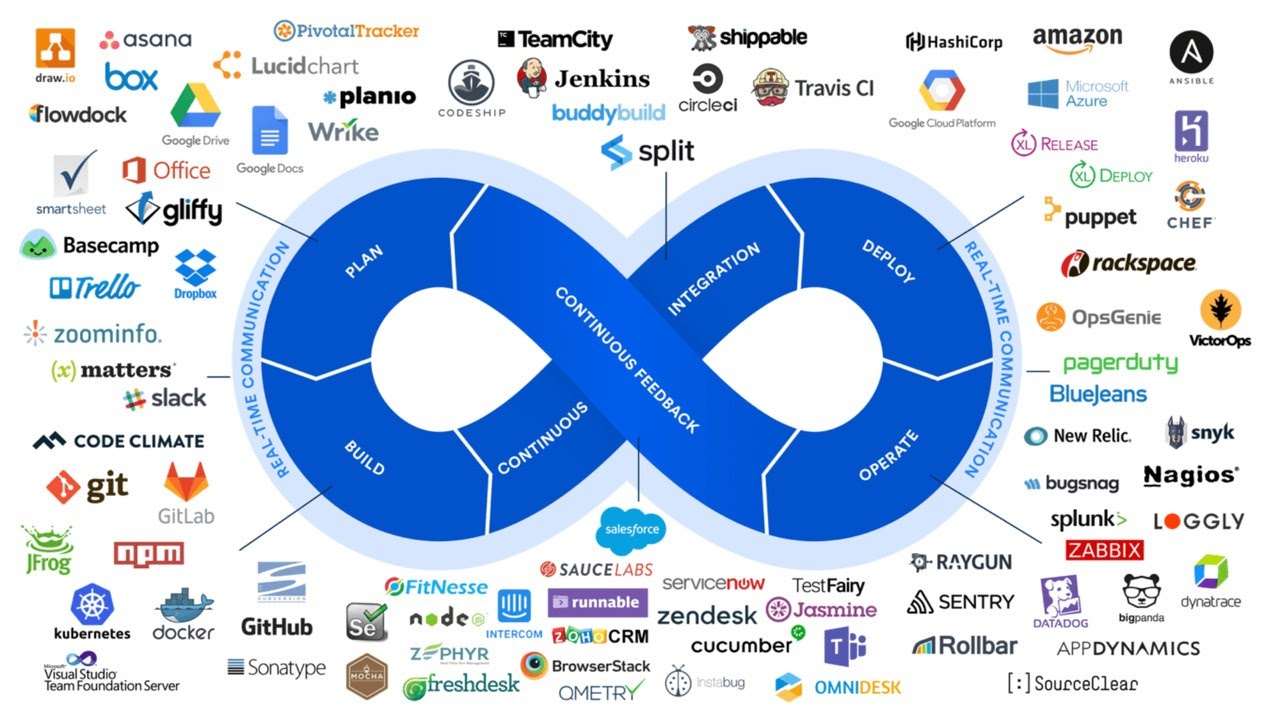
\includegraphics[width=\textwidth]{Graphics/devops}
\caption{\ac{DevOps} \cite{uplink:2021}}
\end{figure}

\section{Fehlerkulturen}

Die Fehlerkulturen beschreiben die grundlegenden Arten auf die mit Fehlern umgegangen werden kann. Es geht darum als was Fehler betrachtet werden, also als etwas Gutes oder Schlechtes, ob sie Strafe mit sich bringen, ein Risiko darstellen und so weiter.

Es gibt prinzipiell innerhalb \ac{DevOps} 2 Fehlerkulturen die im Konflikt zueinander stehen. Diese sehen wie folgt aus:

\begin{description}
\item[Nullfehlertoleranz]\hfill\\ Wie der Name bereits vermuten lässt, sollen hierbei Fehler absolut ausgeschlossen sein. Sie werden immer als etwas Negatives betrachtet, da sie ein Unternehmen Reputation oder Geld kosten können. In schweren Fällen und je nach Anwendungsgebiet, kann ein Fehler sogar ein Leben kosten. Daher ist es unerlässlich, eine solche Nulltoleranz in manchen Fällen walten zu lassen. Folglich sind die Fehler auch oft mit Scham behaftet, und bedeuten für Denjenigen der ihn zu verantworten hat oft eine gewisse Strafe. Dies übt einen großen Druck aus und ist in der Realität nie zu hundert Prozent zu gewährleisten.

Diese strikte Umgangsart mit Fehlern regt natürlich auch dazu an, möglichst bei Altbekanntem zu bleiben, und keine Experiment zu wagen. Dabei ist natürlich kein großer Raum für Fortschritt.

Um diese Freiheit von Fehlern zu gewährleisten, fallen oft auch weitere Kosten an, beispielsweise für weitere spezialisierte Tools, oder mehr Personentage um ausgiebiger testen zu können. Andererseits sollen hierbei auch einfach Missverständnisse und Fehler durch den letztendlichen Anwender vermieden werden, der vielleicht das Interface nicht eindeutig oder intuitiv genug zu bedienen findet. Stichwort Human Computer Interaction.


\item[Experimente erlauben]\hfill\\ Auch diese Begrifflichkeit ist selbsterklärend. Fehler sind hierbei nicht nur weniger schlimm als bei der Nullfehlertoleranz, sie werden sogar offen begrüßt und sind erwünscht. Ein Fehler ist hierbei nicht typischerweise schambehaftet.

Es geht um ein Trial-and-Error-Mindset, welches zum Experimentieren anregen soll. Denn nur das Experimentieren mit neuen Technologien oder Ideen, bringt auch tatsächlich Fortschritt und kann somit auf langfristige Sicht einen großen Vorteil bedeuten. Denn es kann stets auf neue Entwicklungen und Technologien reagiert werden. \glqq Handeln kann Fehler verursachen; nicht zu handeln kann der größere Fehler sein.\grqq
\end{description}

Die Kunst besteht nun darin, die richtige Fehlerkultur an der richtigen Stelle zu wählen. Sie stehen sich ganz klar gegensätzlich im Weg und können nicht miteinander vereint werden. Daher muss immer abgeschätzt werden, wie schwerwiegend Fehler an einer bestimmten Stelle sein können. Wenn es beispielsweise darum geht, dass ein bemanntes Flugzeug abstürzen könnte wenn ein System ausfällt, dann wird die Nullfehlertoleranz gewählt. Hier werden eindeutig keine Fehler gewünscht und solche können dramatische Folgen haben. In einer kleineren Verwaltungssoftware zum Beispiel hingegen, sind Fehler weniger gravierend und leichter zu beheben. Hier kann also zu Gunsten einer möglichen Verbesserung von Prozessen oder des Systems in der Zukunft experimentiert werden. So eindeutig sind die Fälle jedoch nicht immer. Daher muss der Grad zwischen Verbesserungspotential und möglichen Schäden durch Fehler abgewägt werden.

\section{Kritikpunkte}

\subsection{Nur ein Hype}

Einer der größten, und vielleicht der häufigste Kritikpunkt war die Annahme, dass \ac{DevOps}, genauso wie unzählige andere Hypes in der IT, schon bald an Relevanz verlieren wird und sich herausstellt, dass doch kein größerer Nutzen dahintersteckt. Allerdings hat sich gezeigt dass die Nutzung und die Präsenz des Themas \ac{DevOps} nicht verringert hat, sondern im Gegenteil immer fester verankert in der heutigen Unternehmenswelt steht. Auch Lean, das dem jetzigen \ac{DevOps} zugrunde liegt, hat sich fest in der Fertigung verankert und ist ein zentraler Bestandteil des Prozesses geworden. Selbiges ist von \ac{DevOps} auch zu erwarten. Die \ac{ITIL} ist der Defacto-Standard wenn es um Service Management geht. Sie stellt einen Best-Practice-Leitfaden dar und hier wurden bereits \ac{DevOps} Anregungen und Konzepte aufgenommen.

\subsection{\ac{DevOps} funktioniert nicht}

2018 wurde hierzu von Heise ein Artikel veröffentlicht mit dem Titel \glqq \ac{DevOps} funktioniert nicht\grqq \cite{weiss:2018}. Es geht darum, dass \ac{DevOps} seine Versprechen nicht halten kann und in der Praxis einfach nicht zu den gewünschten Erfolgen führt.

Grund dafür ist jedoch nicht, dass \ac{DevOps} an sich nicht funktioniert, sondern dass es, laut dem Artikel, am Management scheitert. Dies ist ein großes Missverständnis das im Kontext zu \ac{DevOps} herrscht. Oft wird davon ausgegangen, dass \ac{DevOps} kaufbar ist. Man stellt jemanden dafür ein, installiert etwas, und dann klappt es. Dies entspricht jedoch nicht der Realität, aus dem einfachen Grund dass es sich bei \ac{DevOps} nicht um ein Werkzeug handelt, sondern viel mehr um die Denkweise und die persönliche Einstellung eines jeden Involvierten.

Wenn das Denken nicht nachhaltig auf \ac{DevOps} angepasst wird, und sich vielleicht nach ein paar Wochen oder Monaten die zum Ziel gesetzten Leitsätze verlaufen, dann ist das gesamte Vorhaben zum Scheitern verurteilt. Dies ist laut einer Studie der \ac{IDC} \cite{idc:2020} auch der am häufigsten angegebene Grund des Scheiterns, beziehungsweise das größte Hindernis bei der Einführung von \ac{DevOps}

\subsection{Silos sind jetzt Andere}

\subsection{•}
